\documentclass[a4paper,12pt]{article}

\usepackage{graphicx}
\usepackage{amsmath}
\usepackage{hyperref}
\usepackage{caption}
\usepackage{subcaption}
\usepackage{circuitikz}

\title{\textbf{Lab Report: Experiment 2}}
\author{EE24BTECH11003 : Akshara Sarma Chennubhatla\\EE24BTECH11005 : Arjun Pavanje}

\begin{document}
\maketitle
\begin{center}
	\textbf{Experiment:}\\Connecting an RC Circuit\\giving Square Wave Input\\plotting Steady and Transient state\\on an Oscilloscope\\for $3$ cases
\end{center}
\vspace{30pt}
\begin{figure}[h!]
	\centering
	
\includegraphics[width = 100pt]{.logo/logo.png}\\
\end{figure}
\vspace{50pt}
\begin{center}
Bachelor of Technology\\
\vspace{10pt}
Department of Electrical Engineering\\
\end{center}
\newpage
\section*{Objective}

To analyze the transient and steady-state responses of an RC circuit to a square wave input $(0-5V)$ in three cases: \newline
\begin{enumerate}
  \item $RC << T$\\
  \item $RC = T$\\
  \item $RC >> T$
\end{enumerate}
where $T$ is the time period of the input square wave.


\section*{Equipment Used}
\begin{itemize}
  \item Function generator
  \item Resistor \(R\)
  \item Capacitor \(C\)
  \item Oscilloscope
  \item Wires
\end{itemize}


\section*{Theory}

\section*{Procedure}

\subsection*{Connecting Circuit}
\pagebreak
Circuit should be of the below form,
\begin{figure}[h!]
    \centering
    \begin{circuitikz}
        \draw
        (0,0) node[ground] {}
        to[vsourcesin, l=\(\pm 5V\)] (0,3) -- (1,3)
        to[R, l=\(R\)] (3,3)
        to[short] (3,2)
        to[C, l=\(C\)] (3,0) -- (0,0) {}
        (3,2) -- (5,2)
        to[R, l=\(r\)] (5,0) -- (0,0);
    \end{circuitikz}
    \caption{RC Circuit}
    \label{fig:circuit}
\end{figure}
\begin{enumerate}
    \item Construct the circuit as shown in the above figures.
    \begin{enumerate}
        \item Connect the positive end of the function generator in series with a resistor
        \item Connect the capacitor and a small resistance in parallel, connect the combination in series with the rest of the circuit.
    \end{enumerate}
    \item Set the function generator to output a square wave with $5V$ amplitude (Peak Voltage $V$, Minimum Voltage $0V$) and a time-period $T$.
    Select the type of cycle as \textit{N-CYCLES}.
    \item Connect the second channel of the function generator to the second channel of the oscilloscope. Set the waveform for this as a square wave with the same conditions as in the first channel. This will allow us to compare output voltage across capacitor with input square wave.
    \item This configuration enables the generation of a square wave with a predefined number of cycles when the trigger button is pressed on the function generator.
    On the oscilloscope, press the \textit{SINGLE} button. This ensures that the next event captured by the oscilloscope is displayed and then the display pauses automatically.
    \item Trigger the burst mode manually on the function generator to generate the single pulse or event.
    \item Observe and record the captured waveforms on the oscilloscope.
    \item To capture steady state, switch from burst mode to continuous mode and capture steady state.
\end{enumerate}

\section*{Results and Verification}
\subsection*{Case 1: \(RC << T\)}
\begin{figure*}[h!]
    {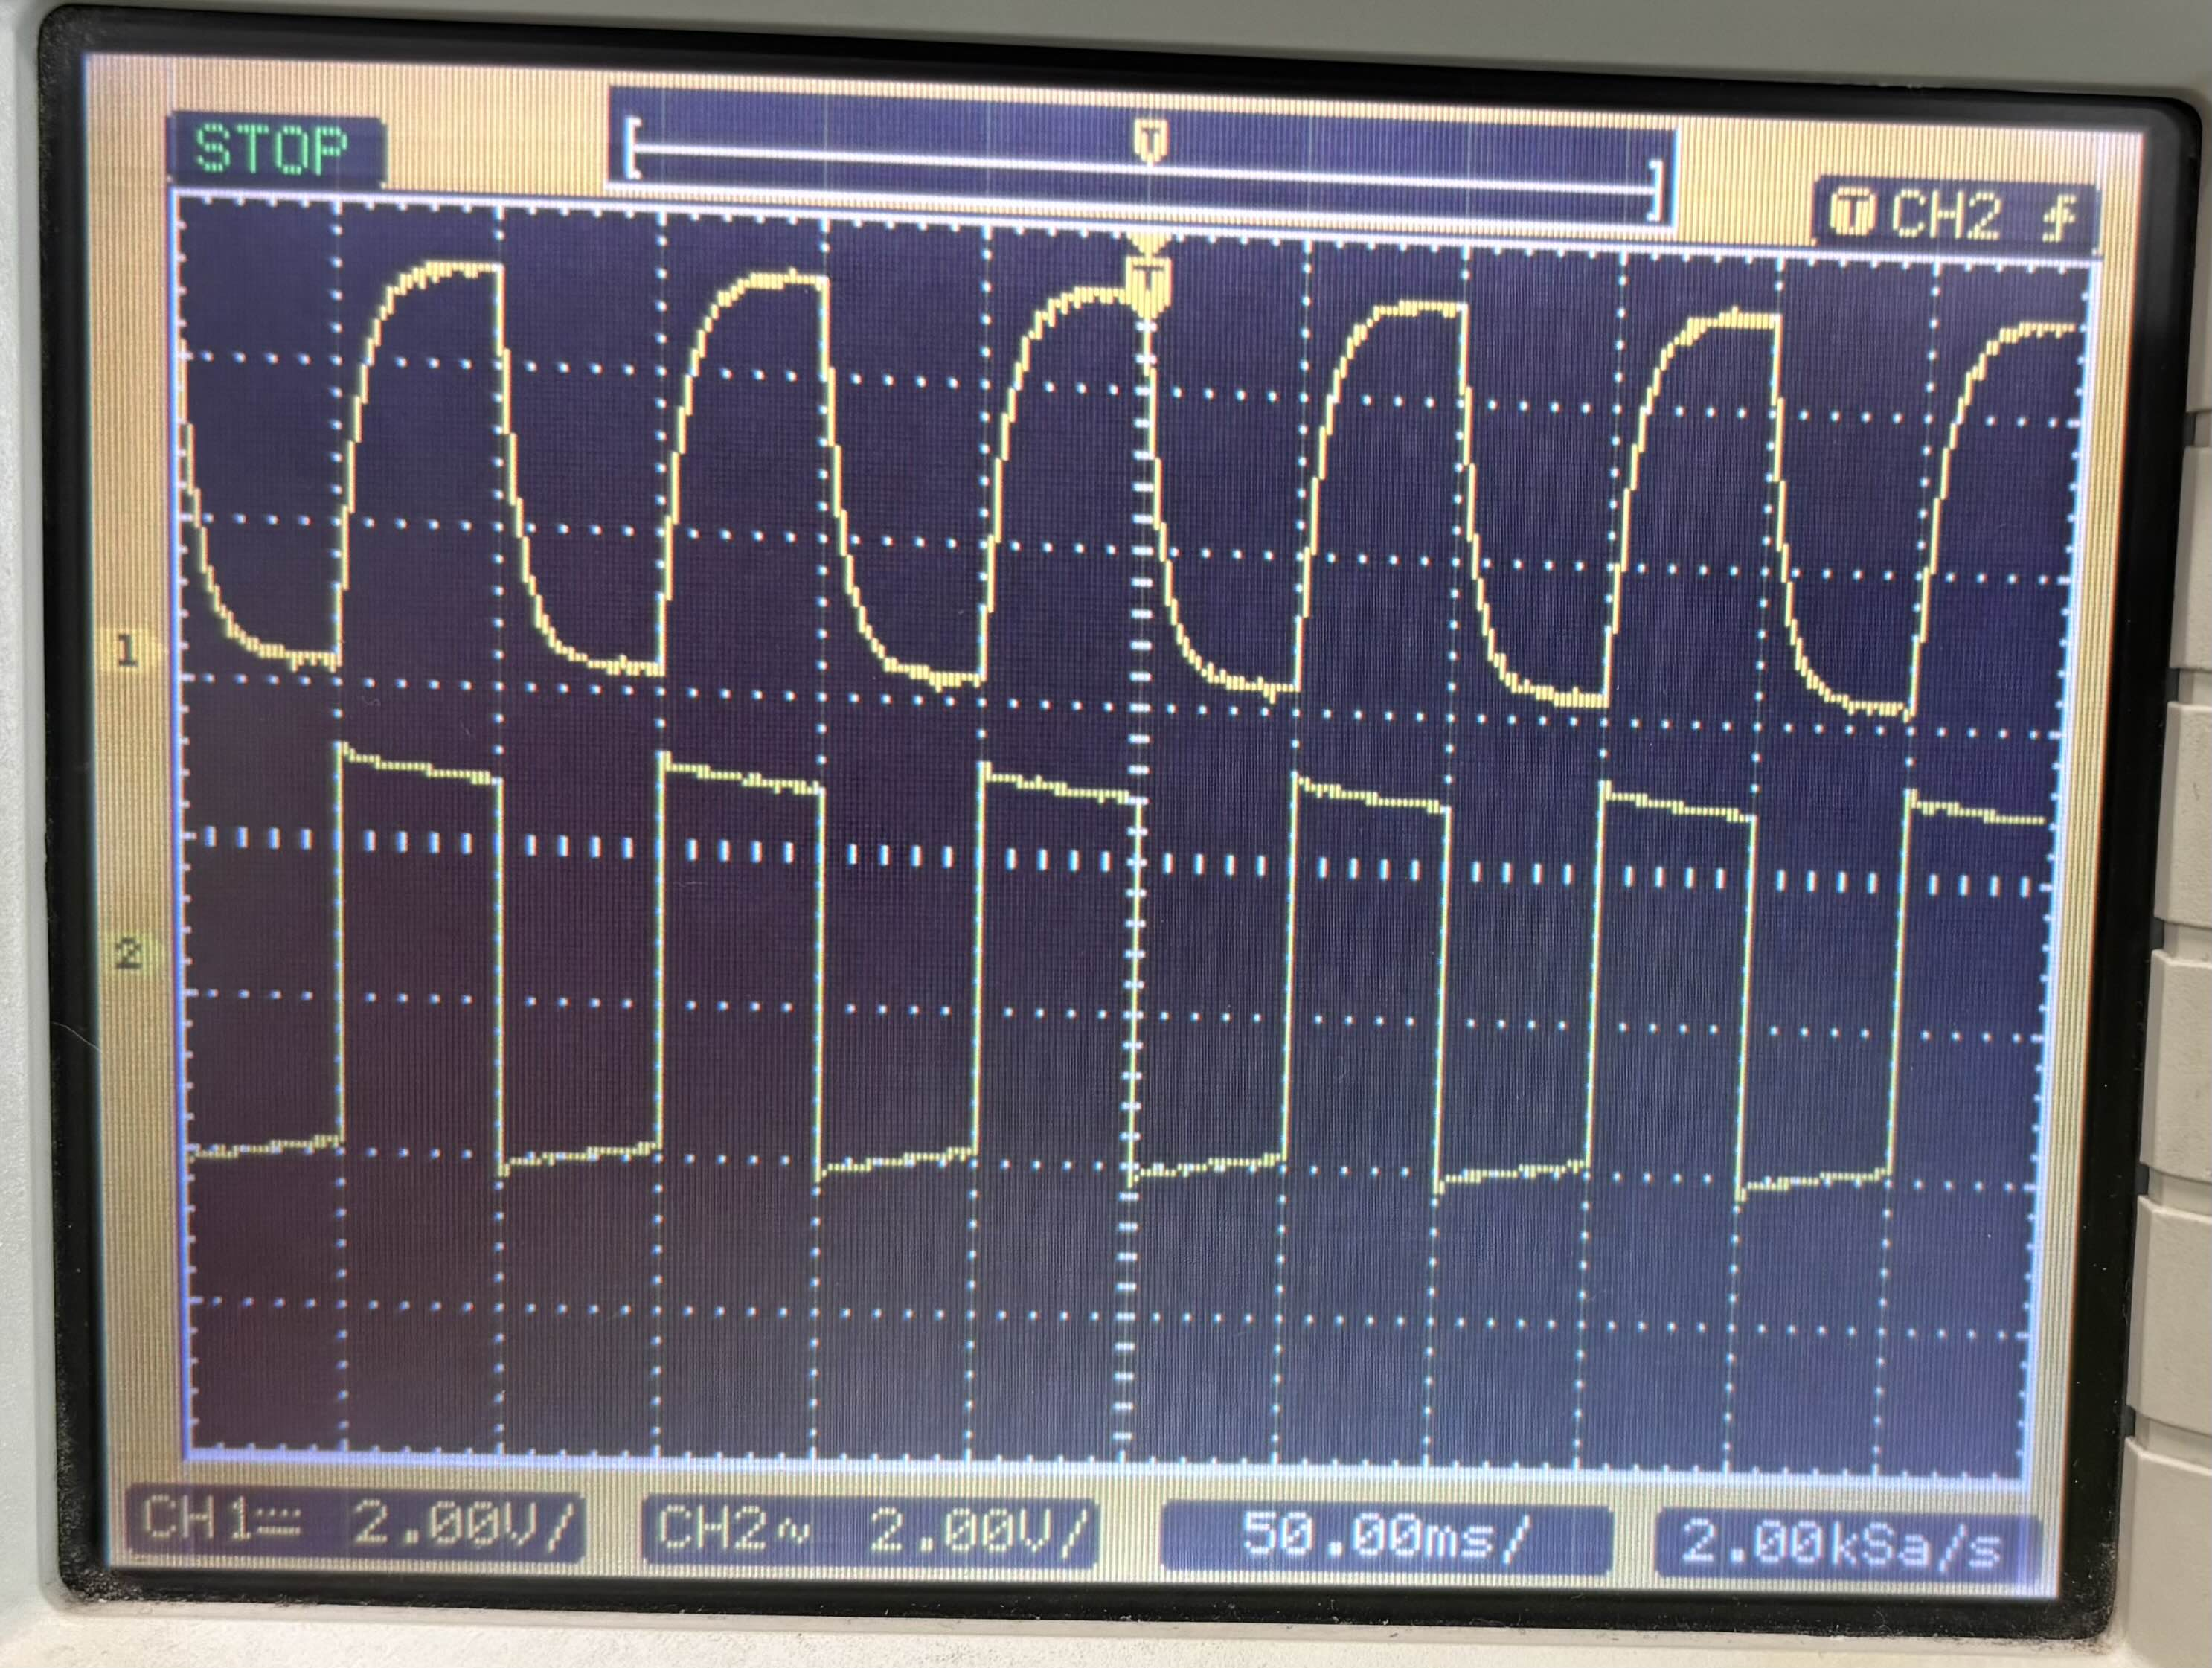
\includegraphics[ width=0.53\columnwidth]{figs/steady_1.jpg}}
    \hspace{\fill}
    {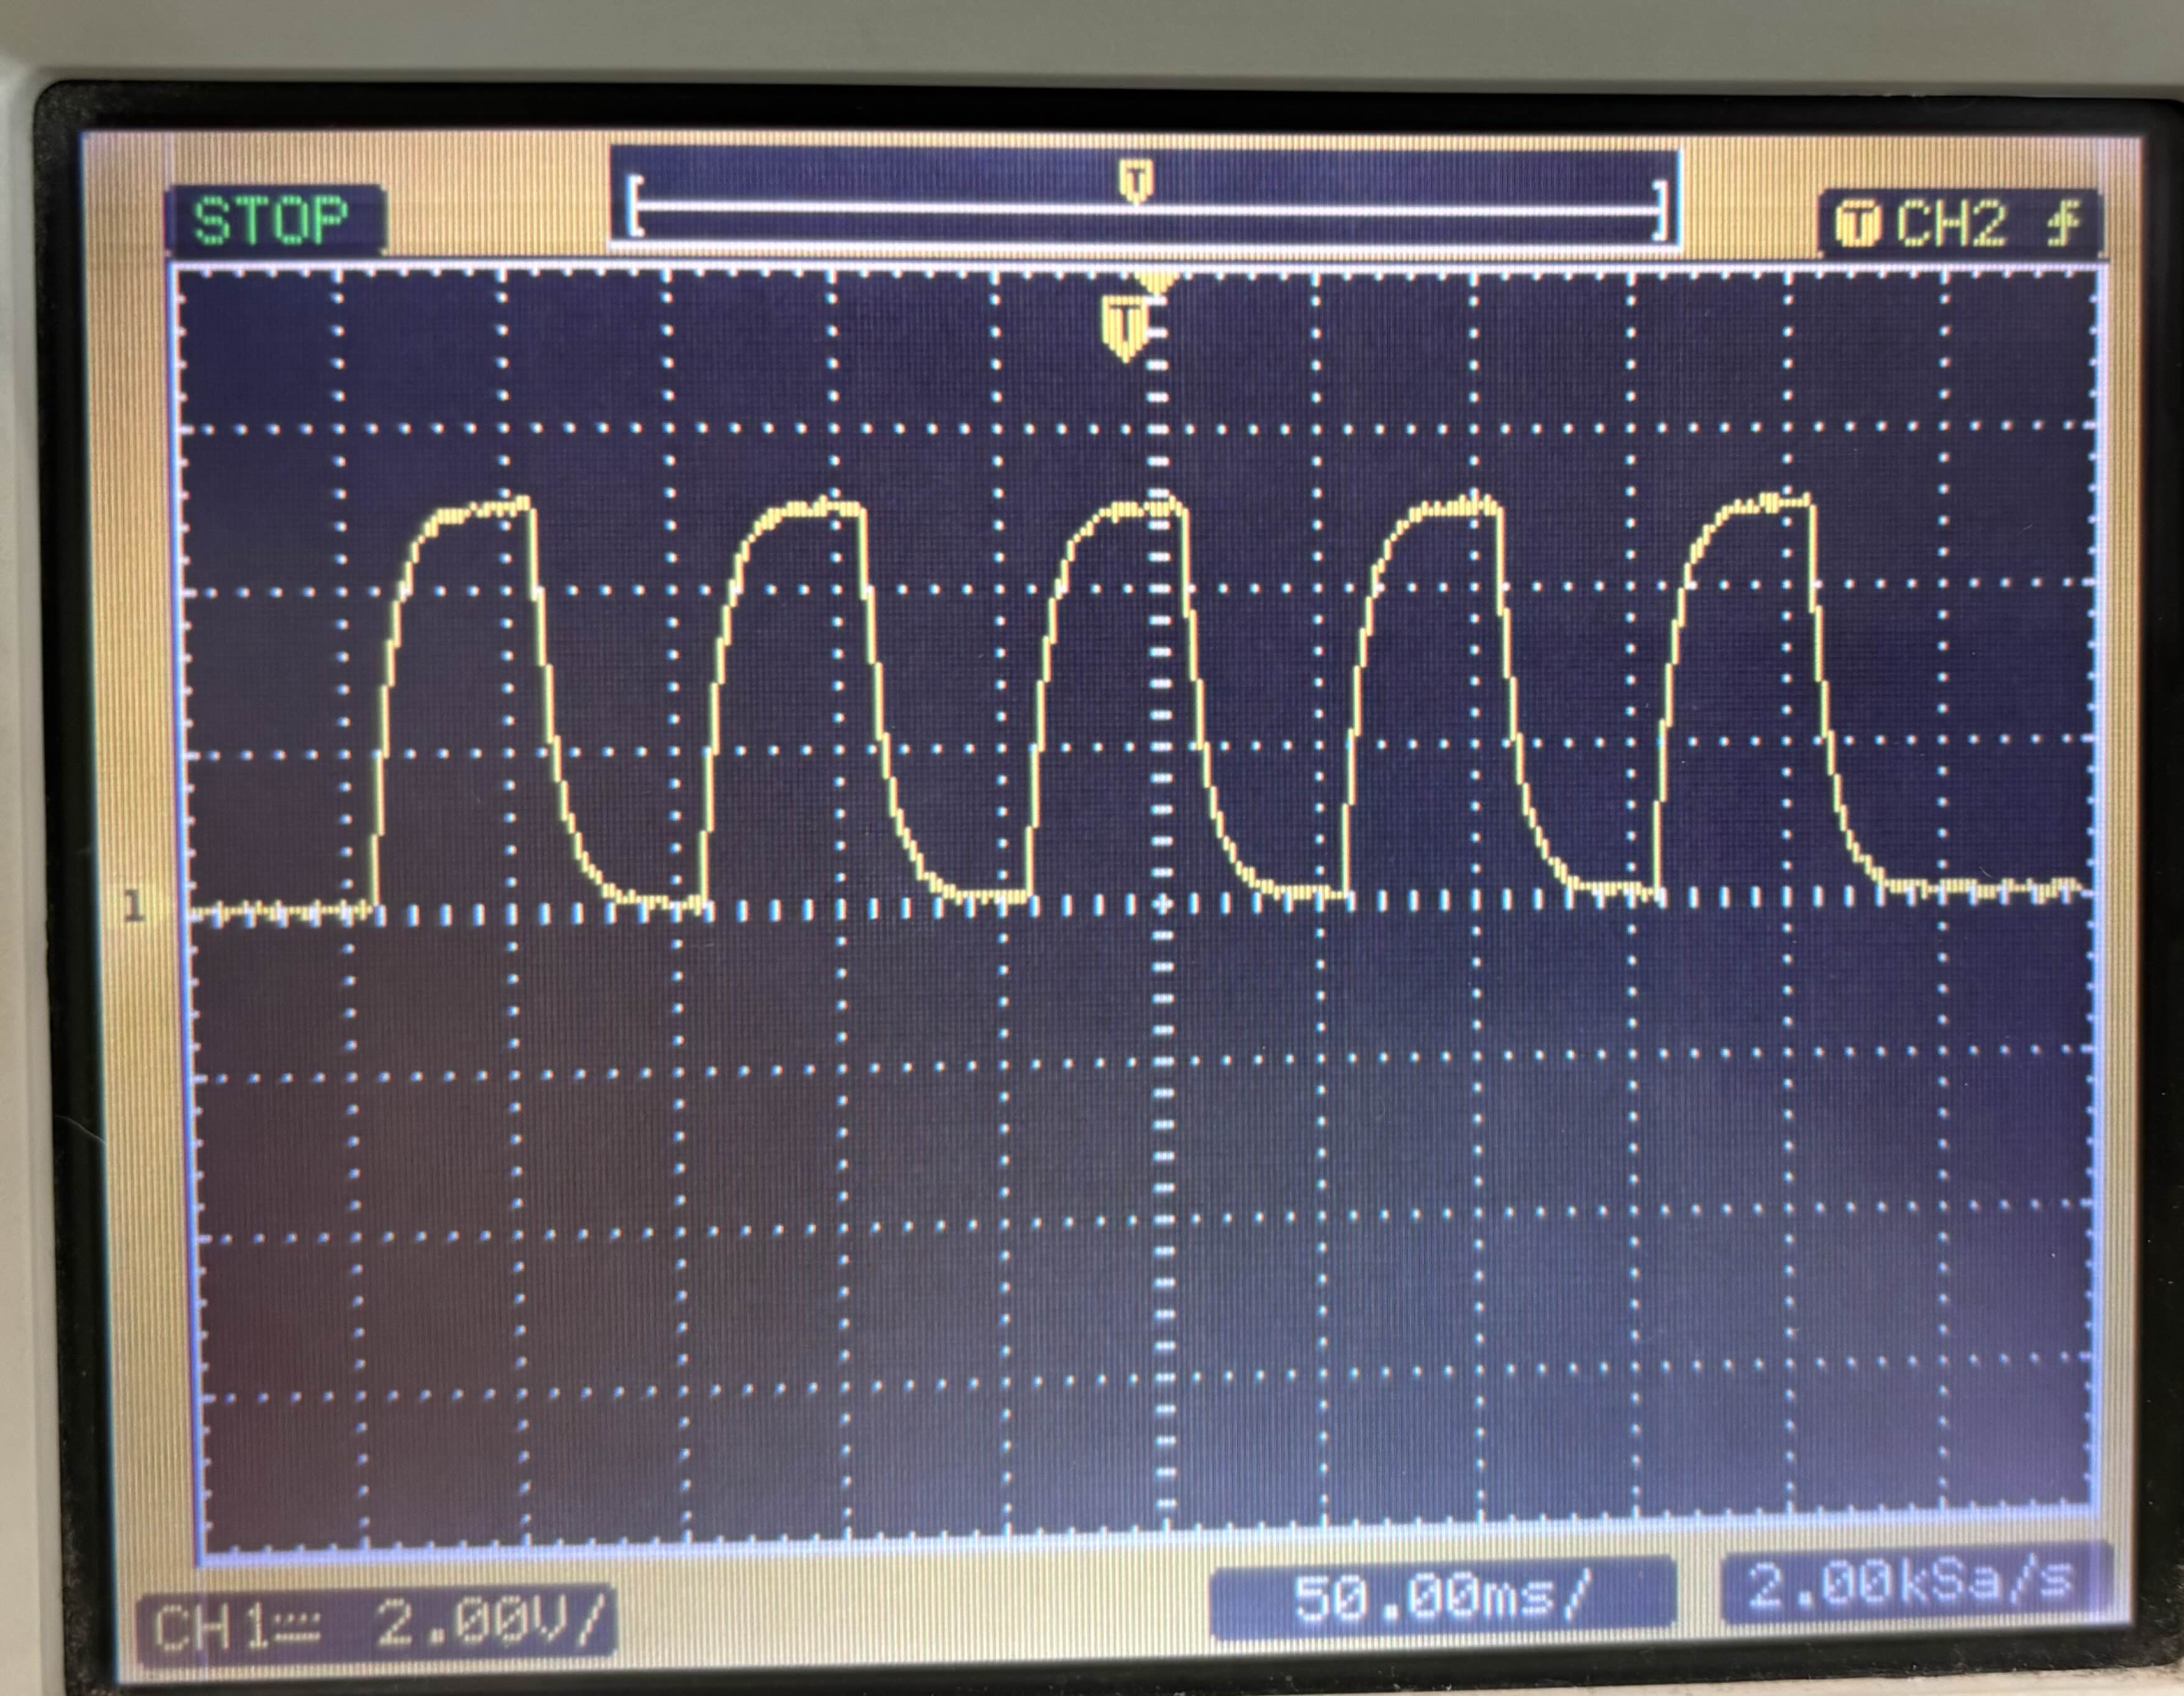
\includegraphics[ width=0.53\columnwidth]{./figs/trans_1.jpg}}
\end{figure*}

\subsection*{Case 2: \(RC = T\)}
\begin{figure*}[h!]
    {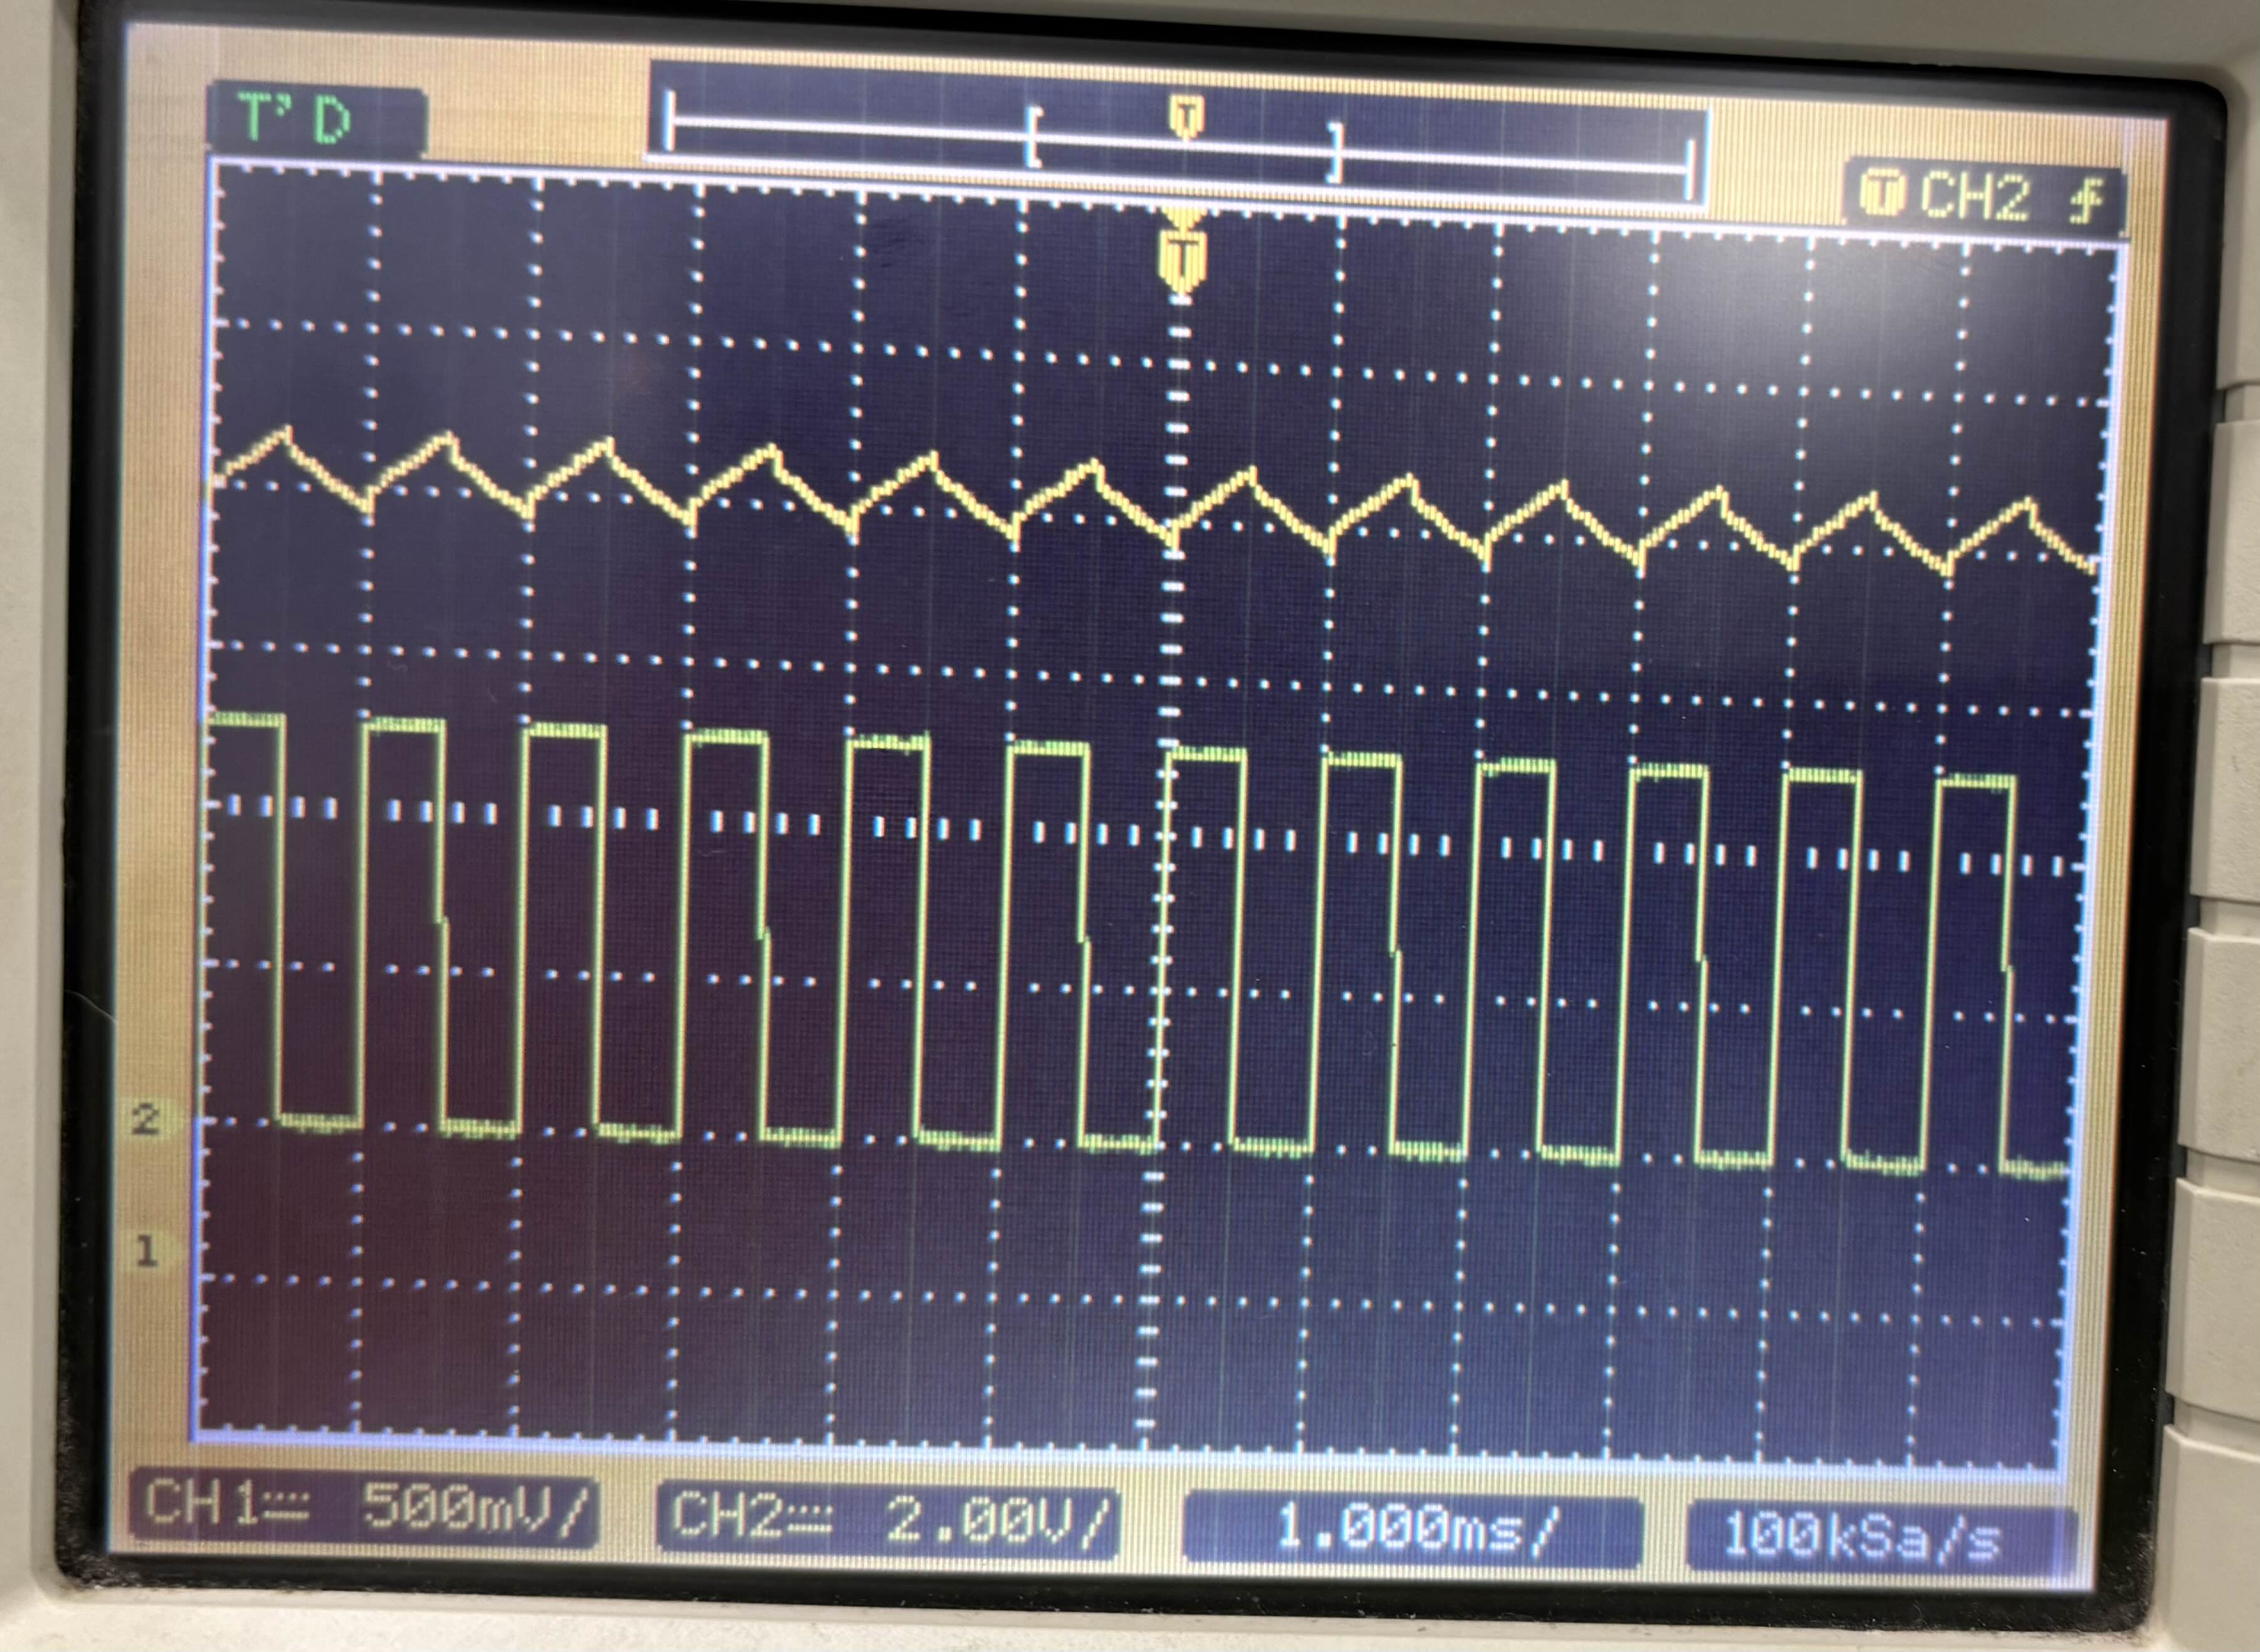
\includegraphics[ width=0.53\columnwidth]{figs/steady_2.jpg}}
    \hspace{\fill}
    {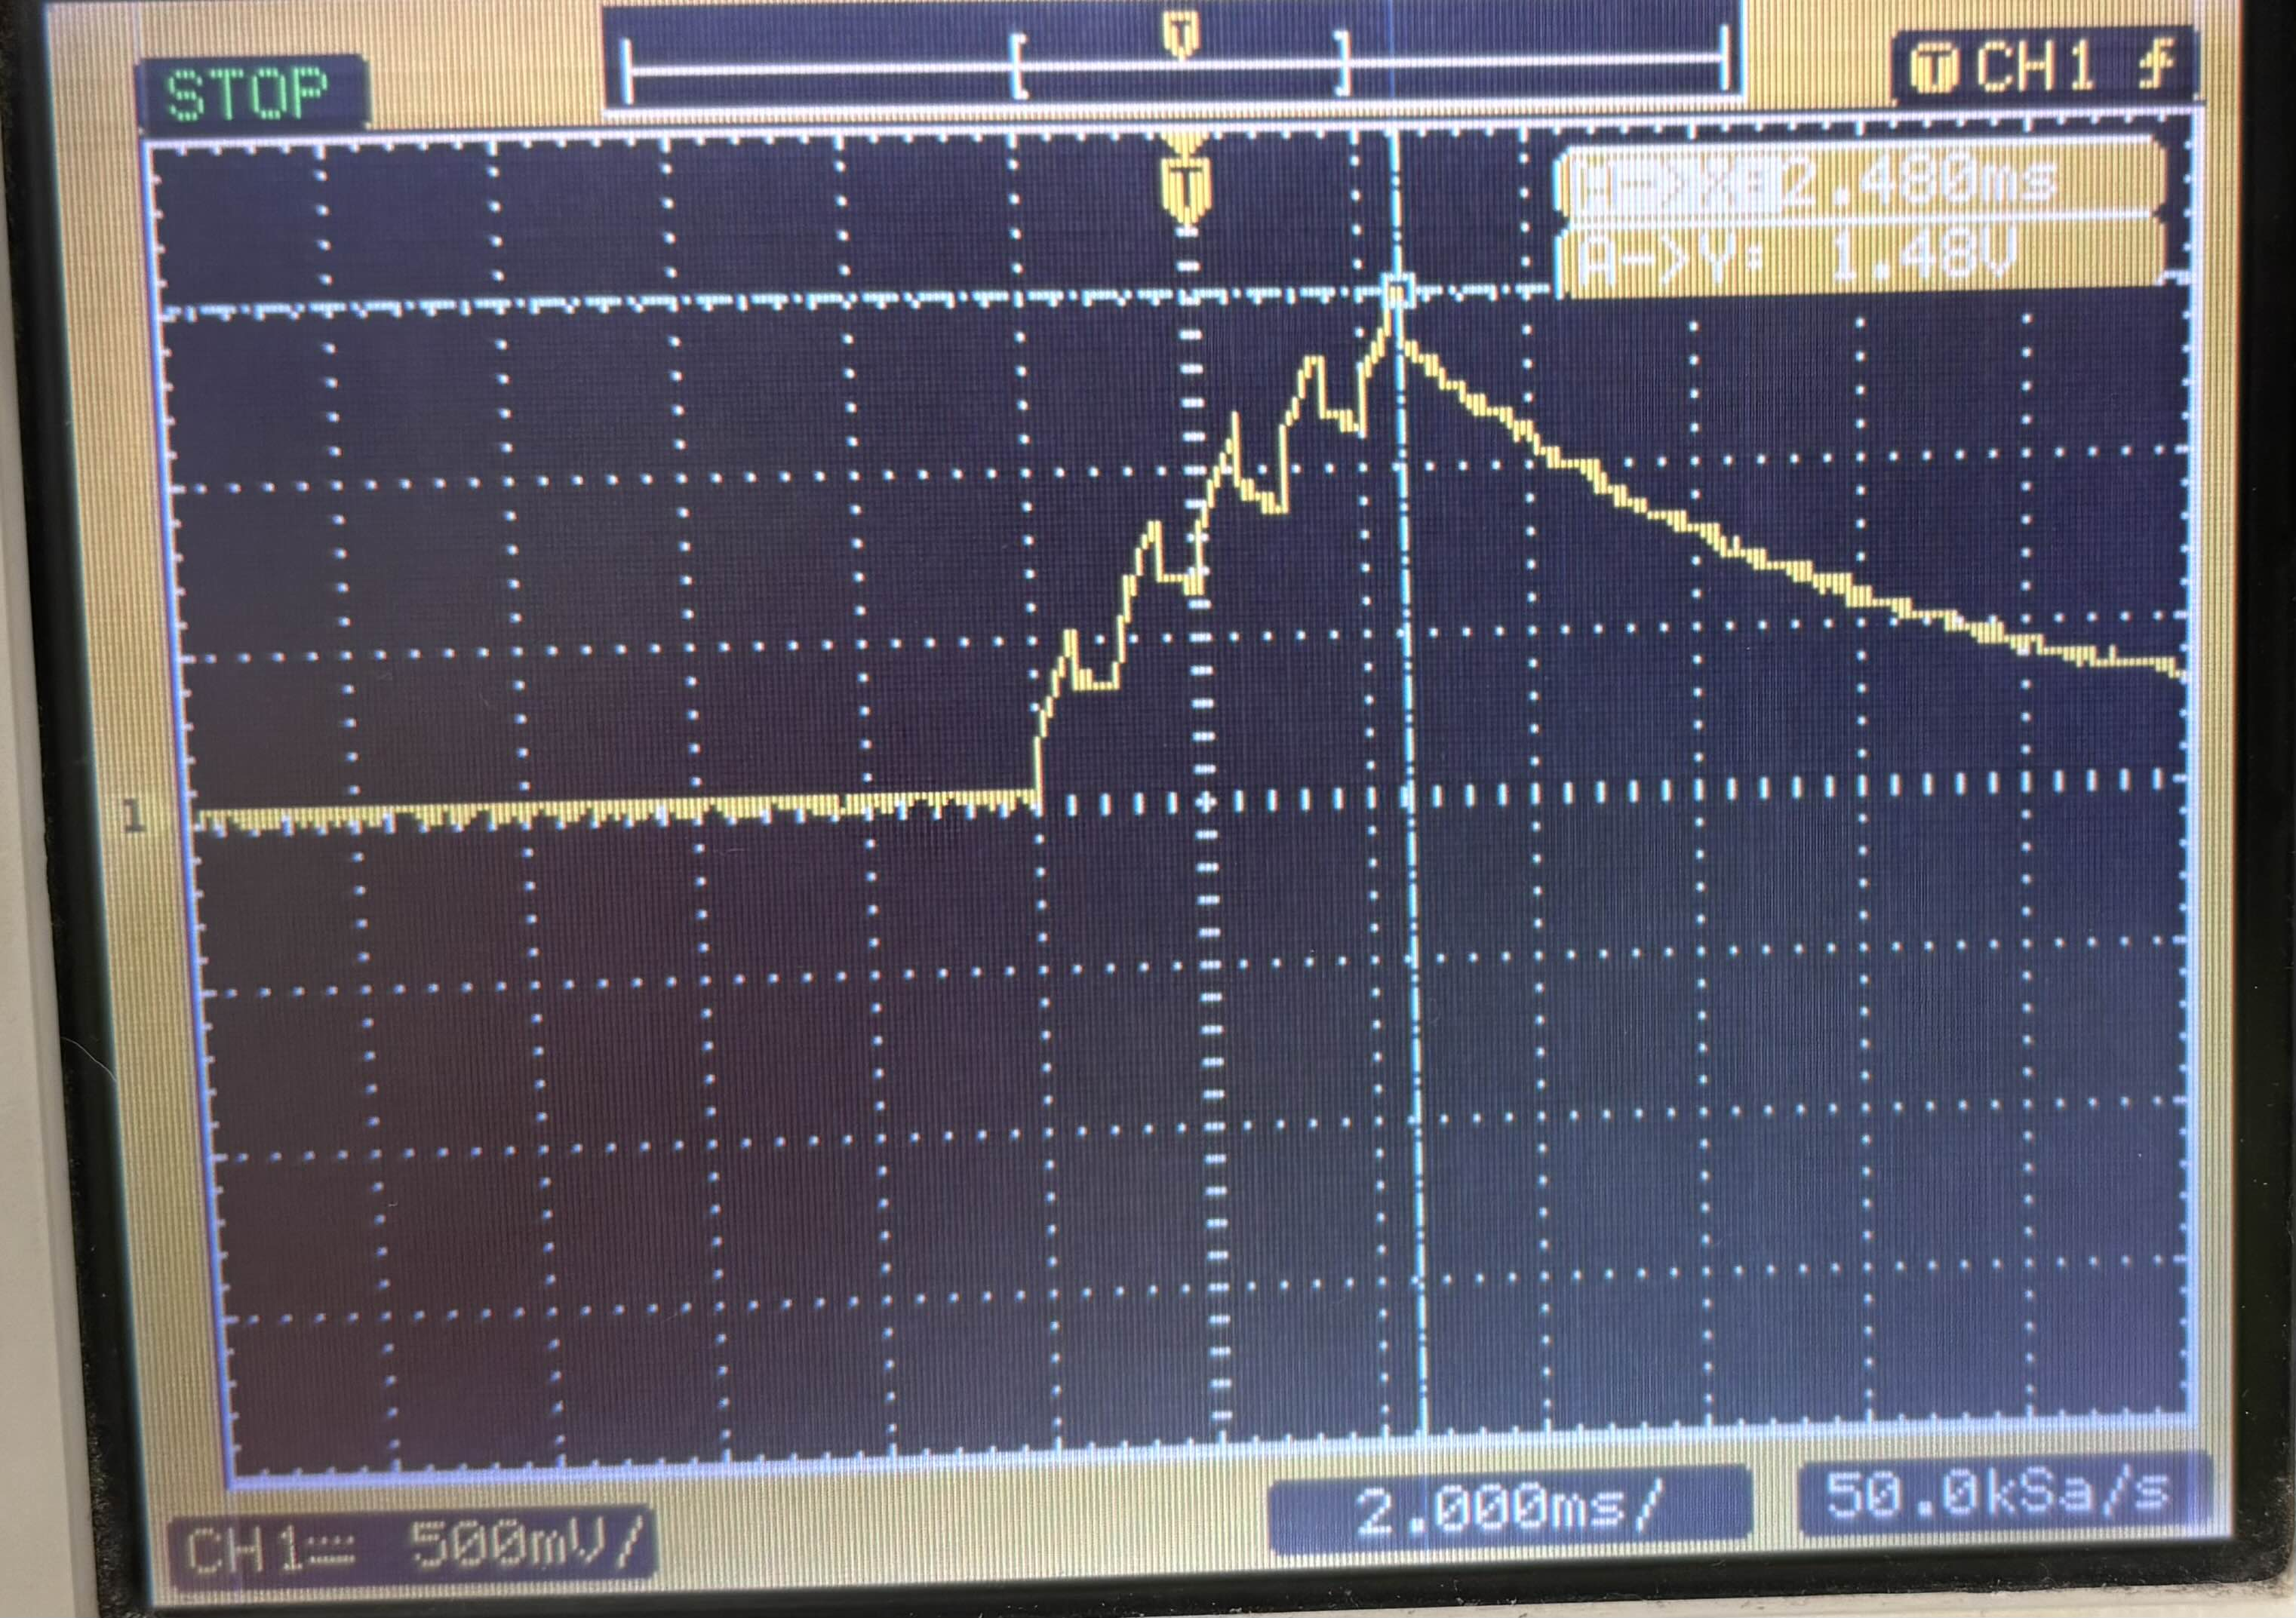
\includegraphics[ width=0.53\columnwidth]{./figs/trans_2.jpg}}
\end{figure*}

\subsection*{Case 3: \(RC >> T\)}
Here, we have plotted more than $5$ cycles of square wave as it better shows the increasing nature of the potential difference across capacitor. 
\pagebreak
\begin{figure*}[h!]
    {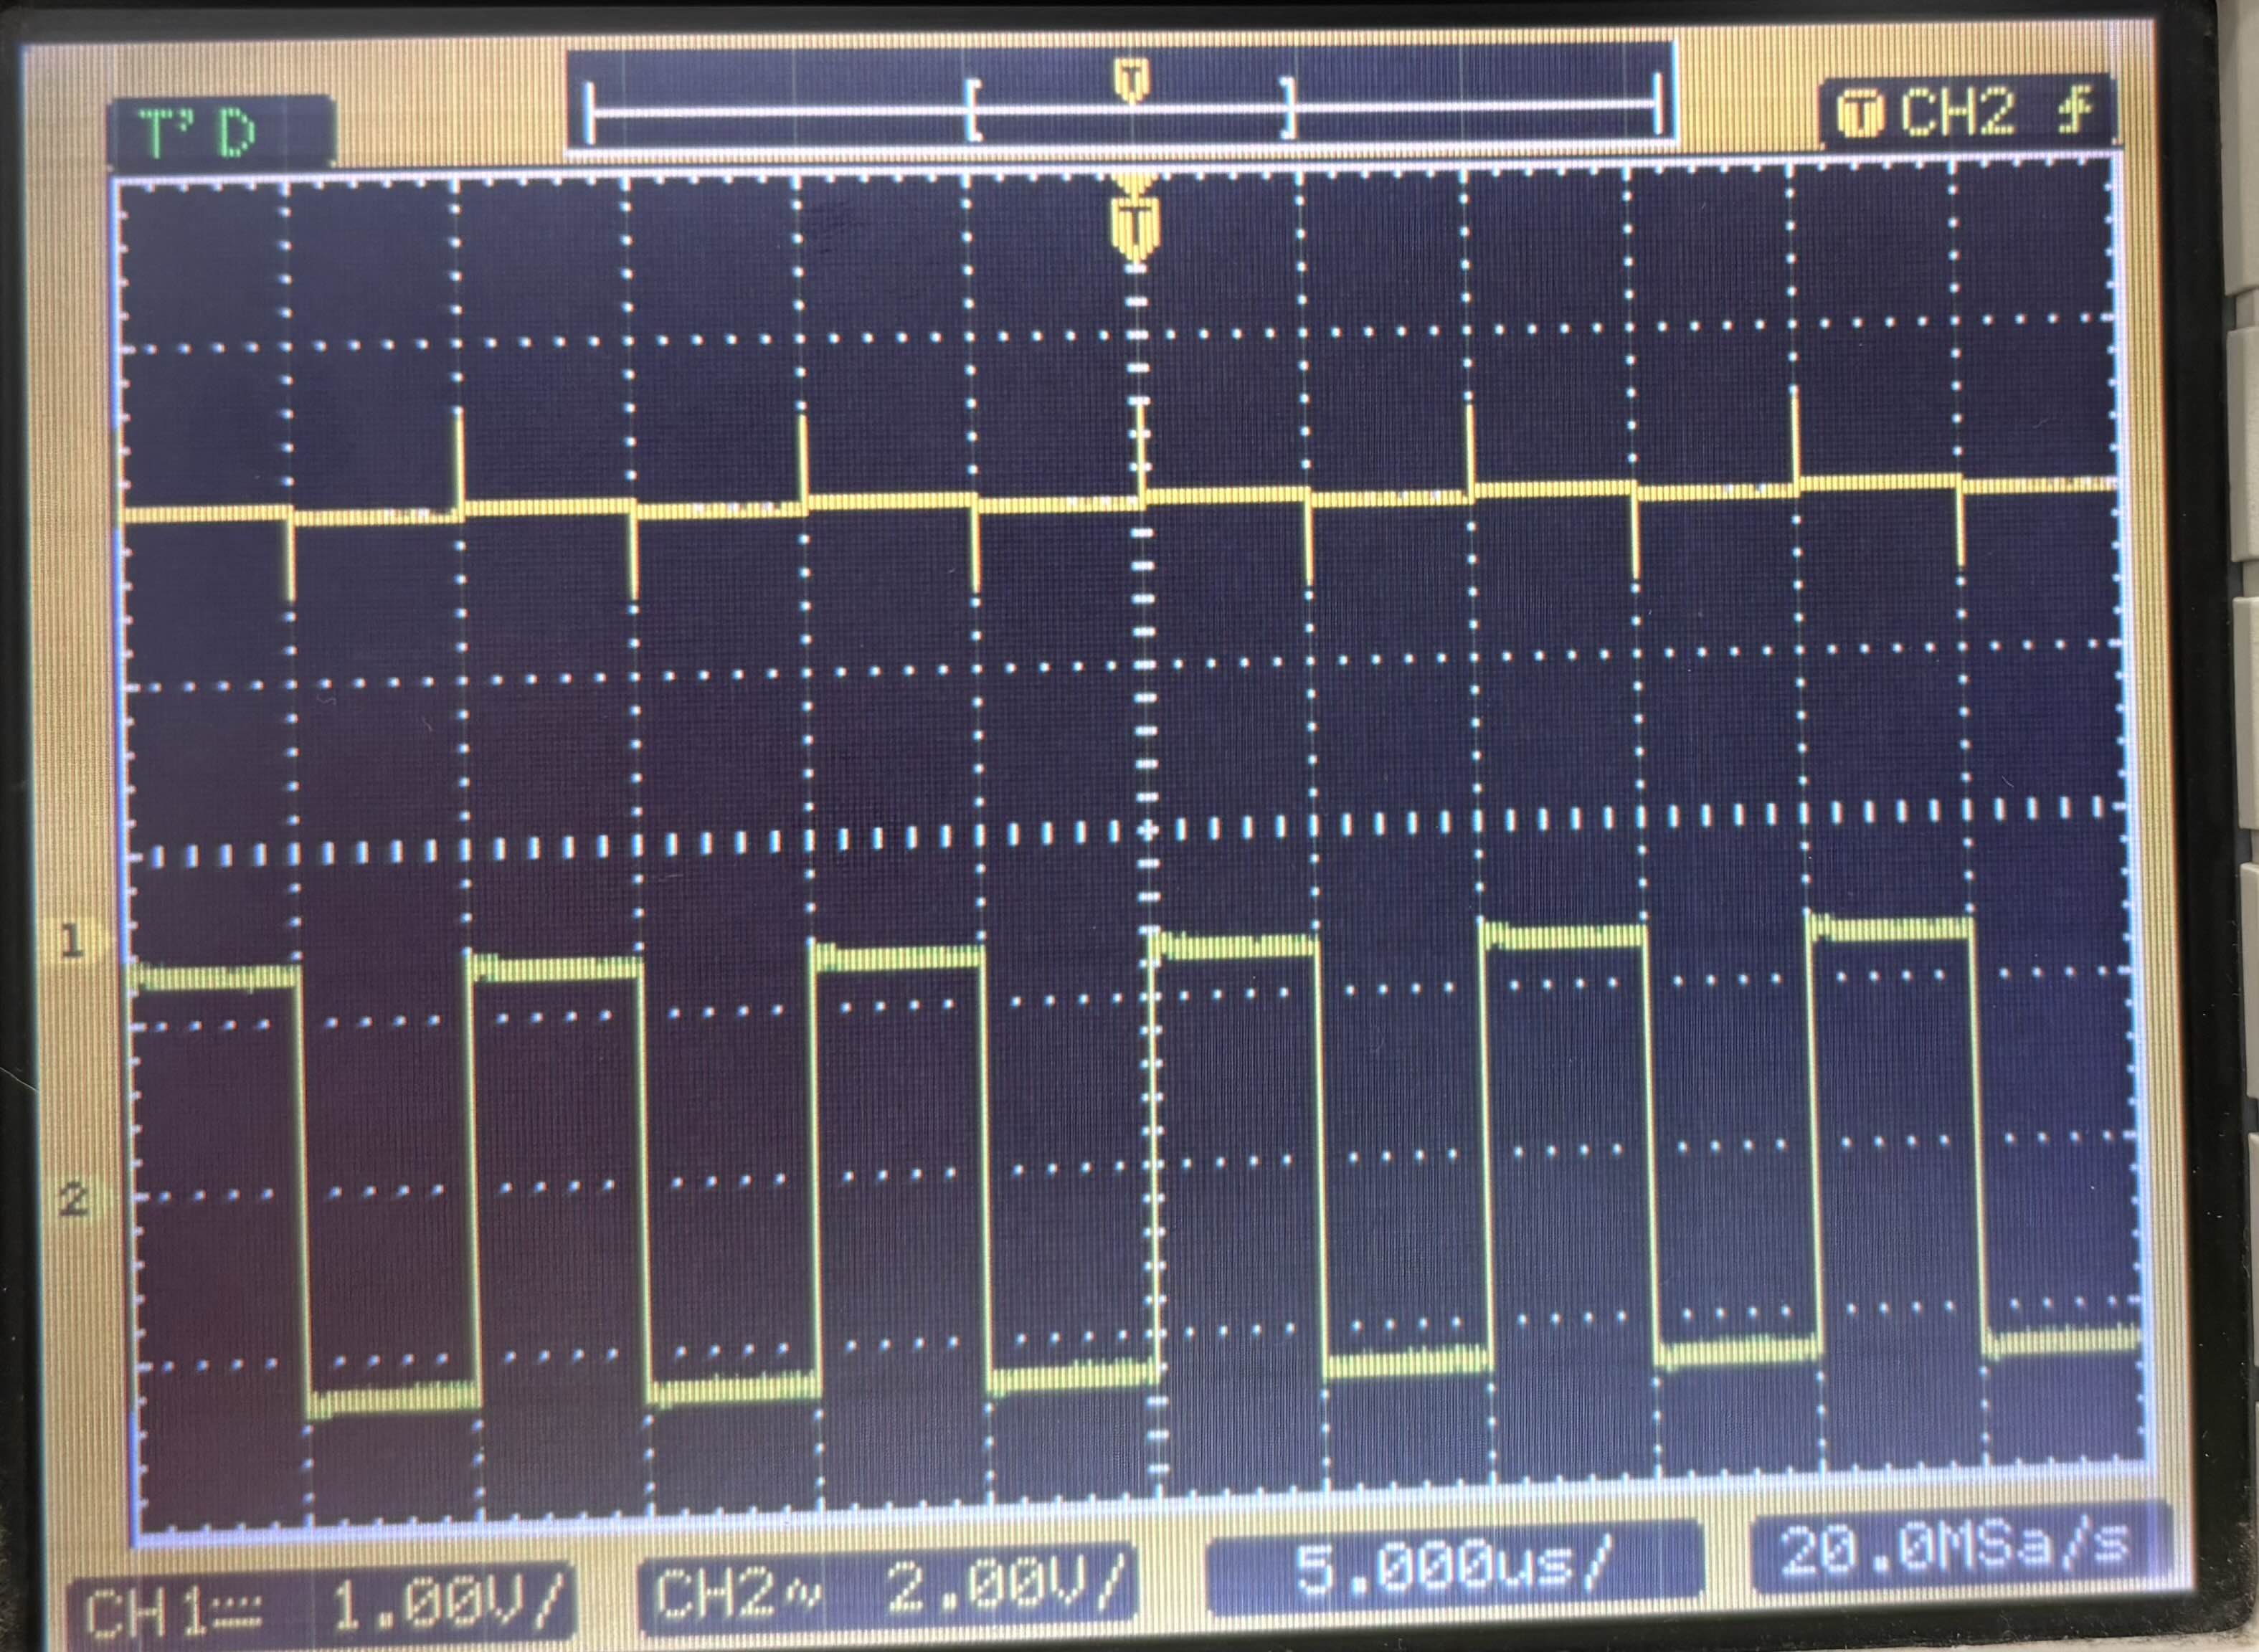
\includegraphics[ width=0.53\columnwidth]{figs/steady_3.jpg}}
    \hspace{\fill}
    {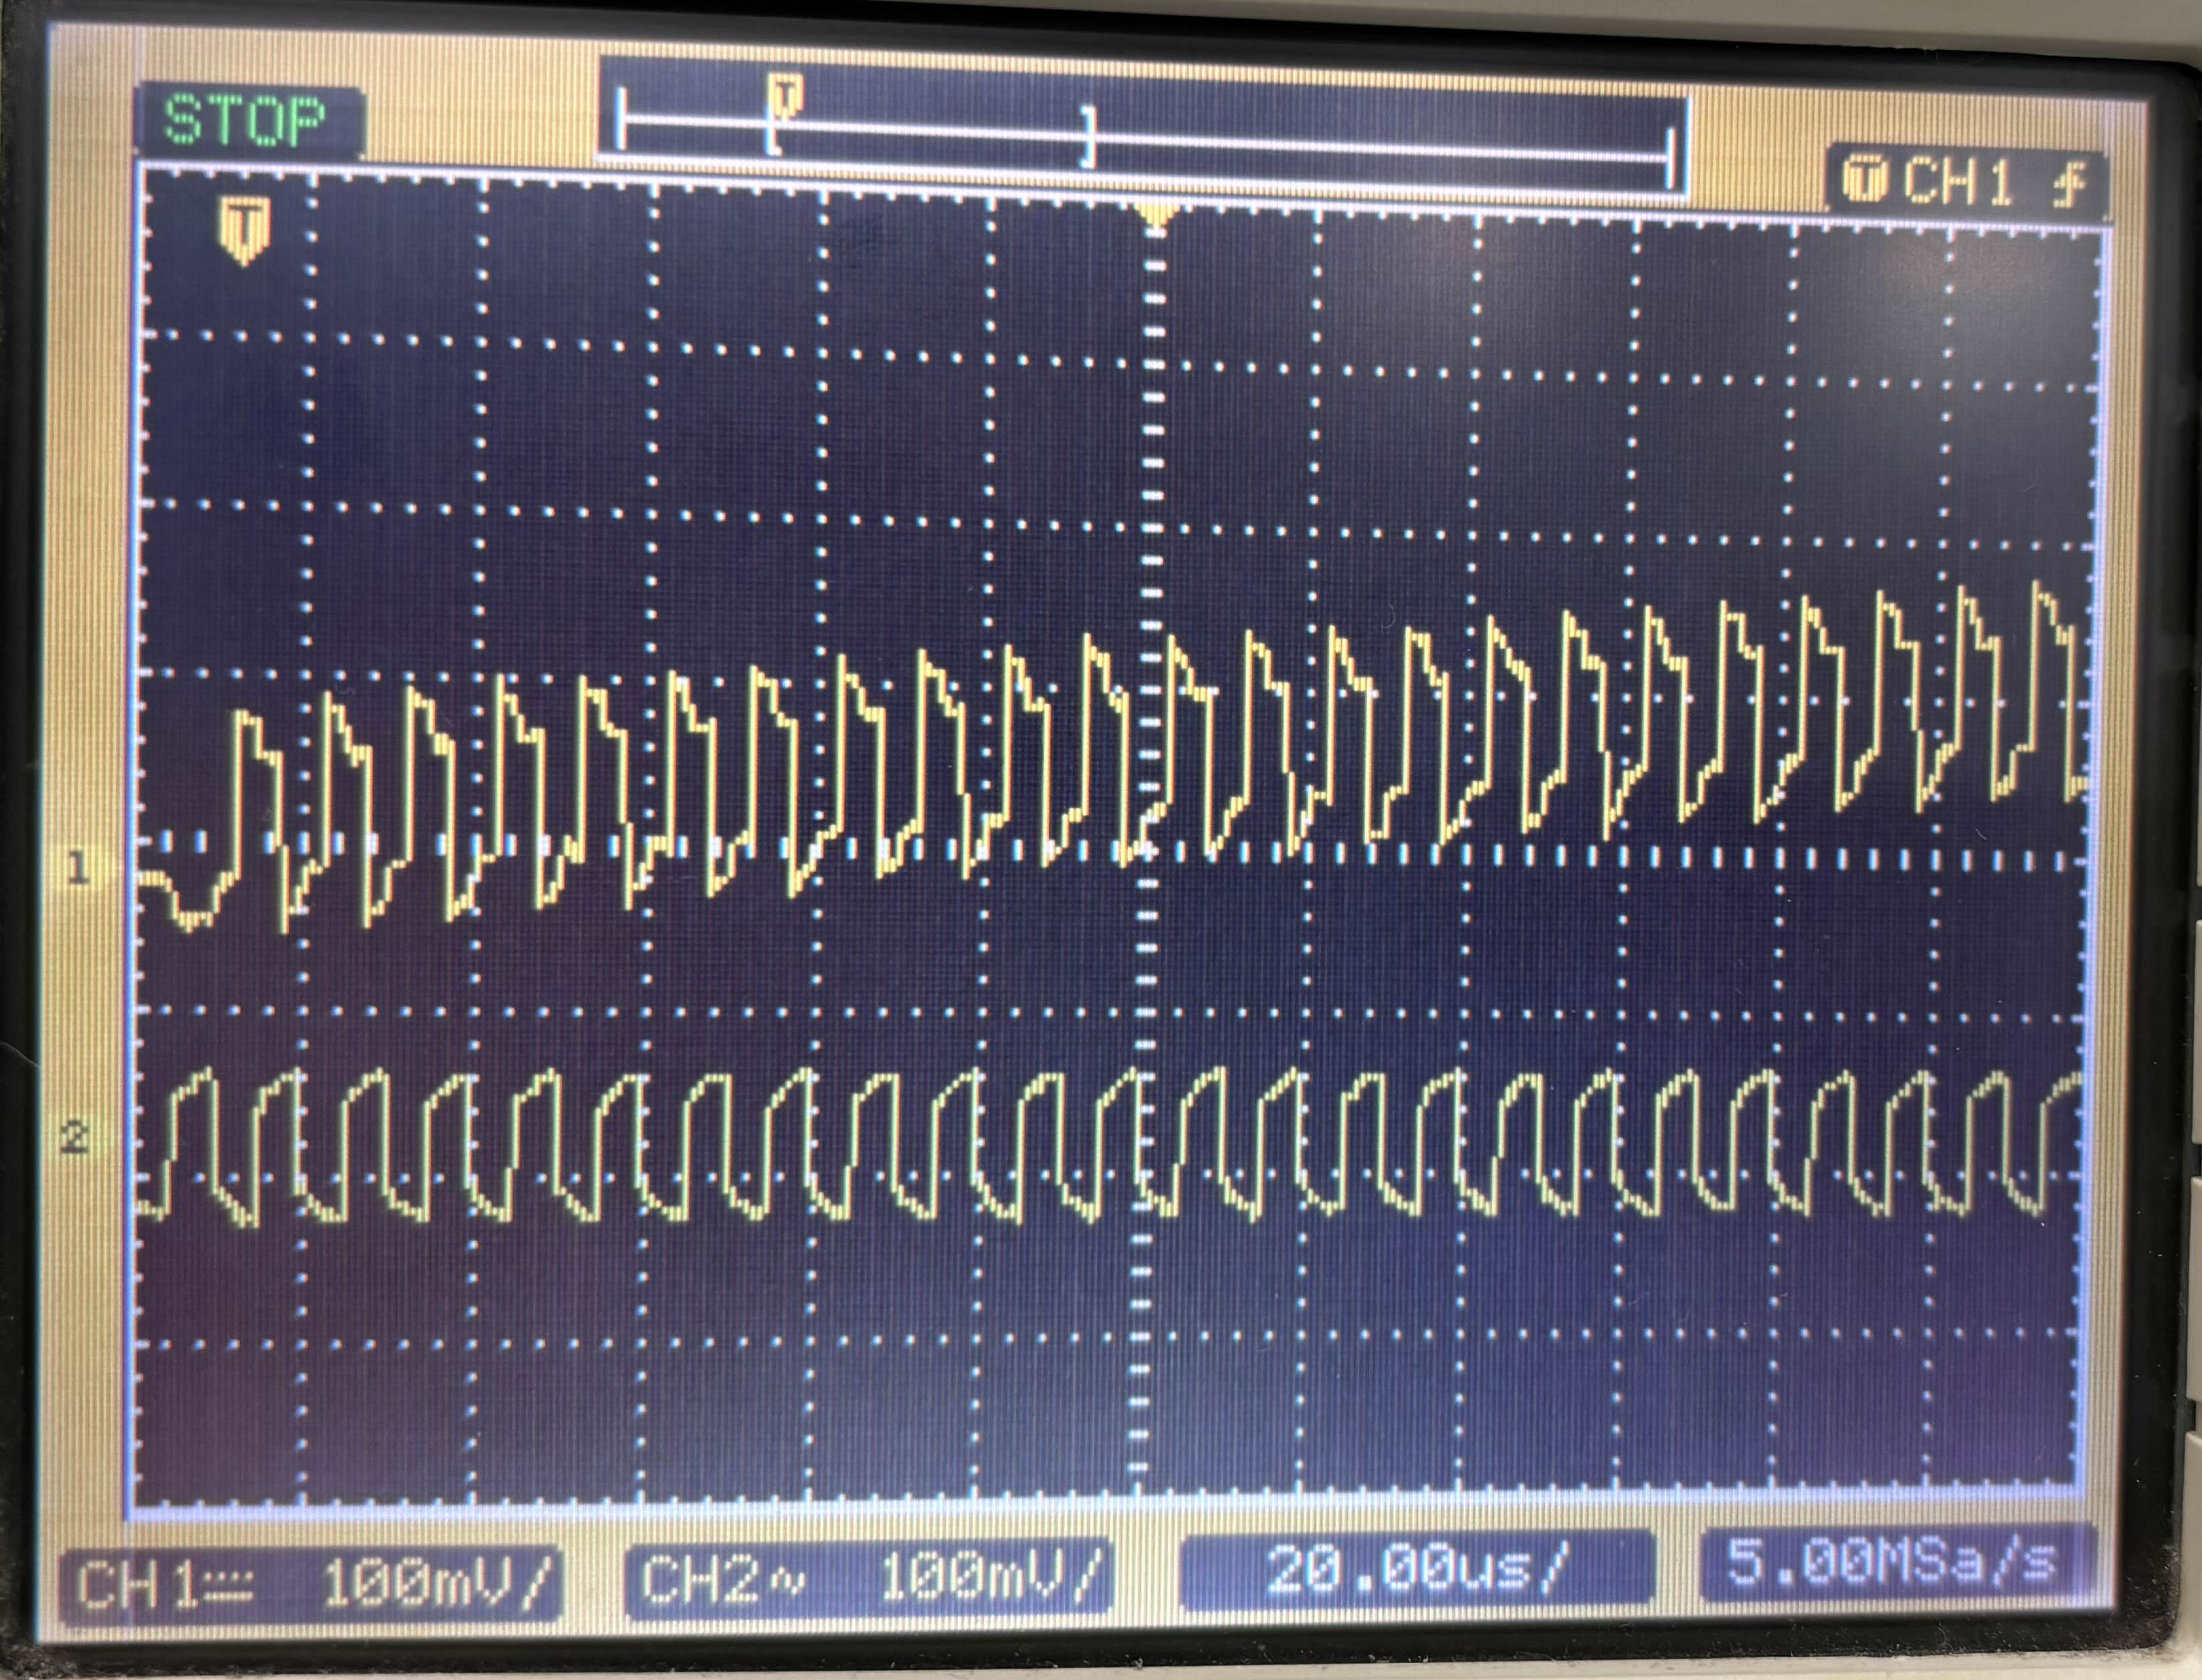
\includegraphics[ width=0.53\columnwidth]{./figs/trans_3.jpg}}
\end{figure*}\\
For an infinite number of cycles of square wave, output comes out to be,
\begin{figure}[h!]
  \centering
  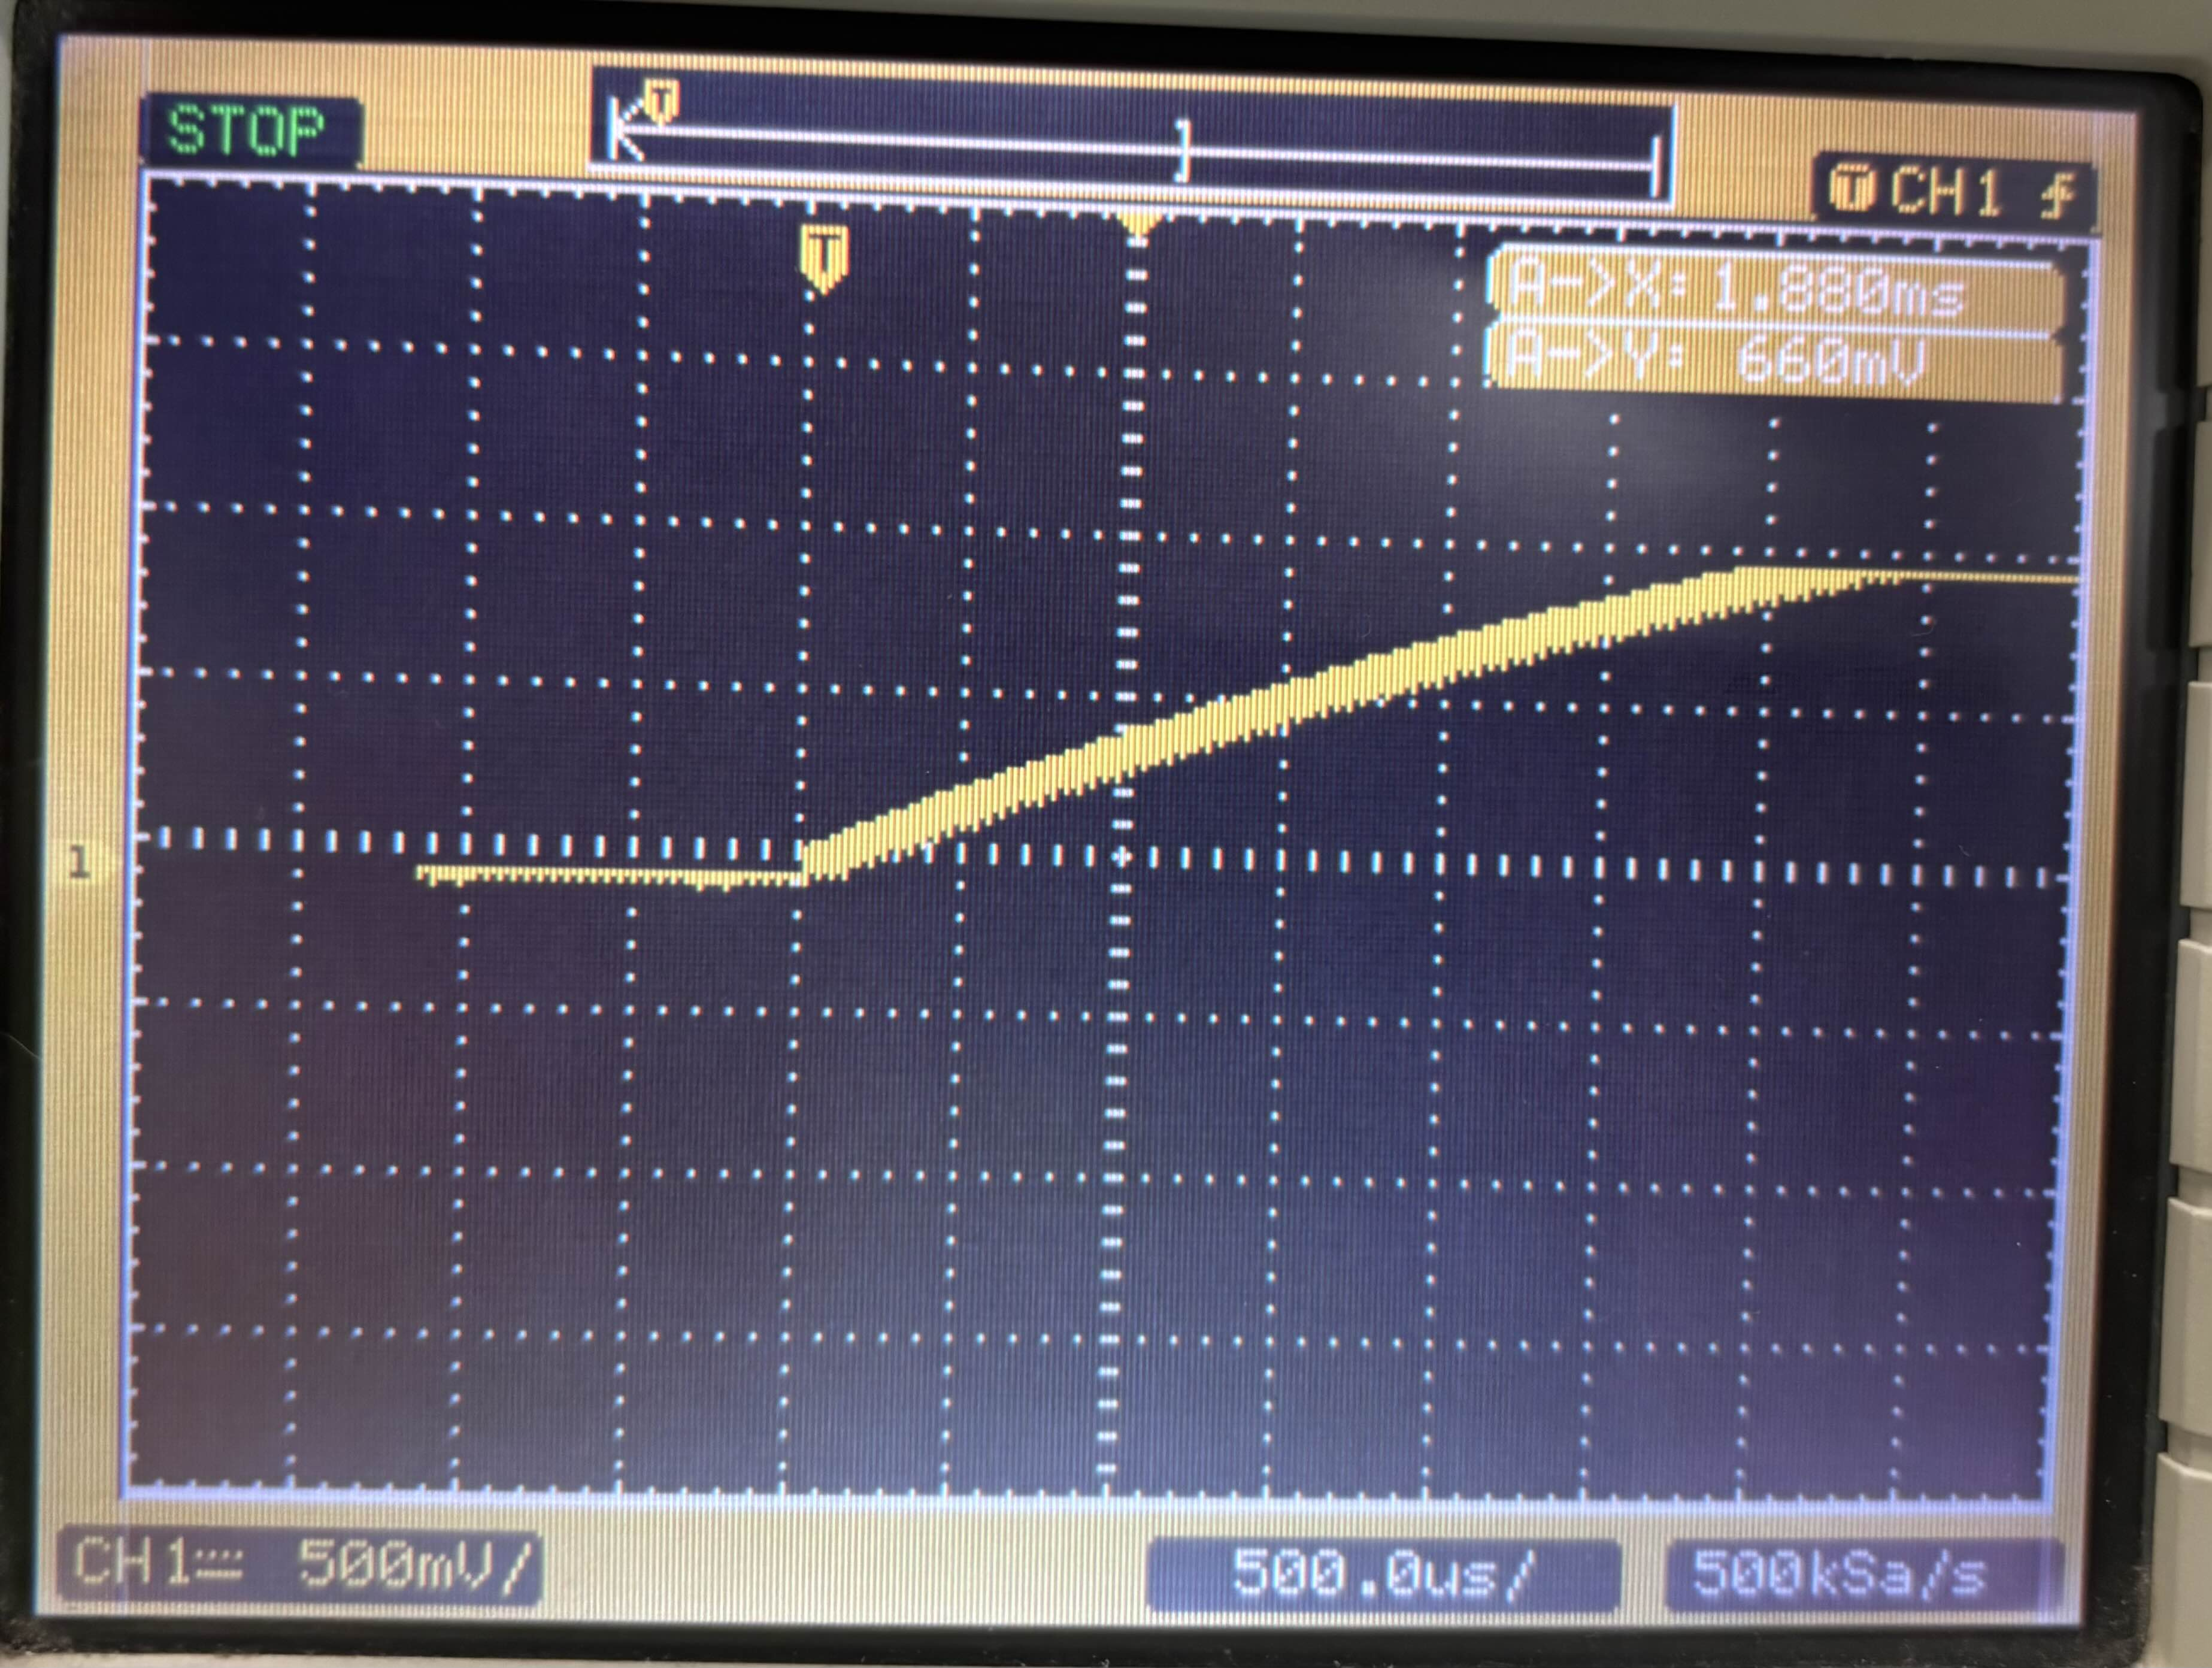
\includegraphics[width=0.7\columnwidth]{figs/trans_infty.jpg}
  \label{label}
\end{figure}\\
Python code verification of obtained graphs:\\
\fbox{\url{https://github.com/ArjunPavanje/EE1200/tree/main/Experiment_2/codes}}

\section*{Conclusion}
We have successfully found and verified the effect (output) of a square wave on a series RC circuit.
\end{document}
